\section{Alloy}
For the evaluation of the model and the elicitation of the requirements we used the specification language \textit{Alloy} which enabled us to express the structural and behavioral constraints of the software system \textit{myTaxiService}.

\lstinputlisting{Appendix/alloy.als}
\pagebreak
\begin{figure}[H]
\centering
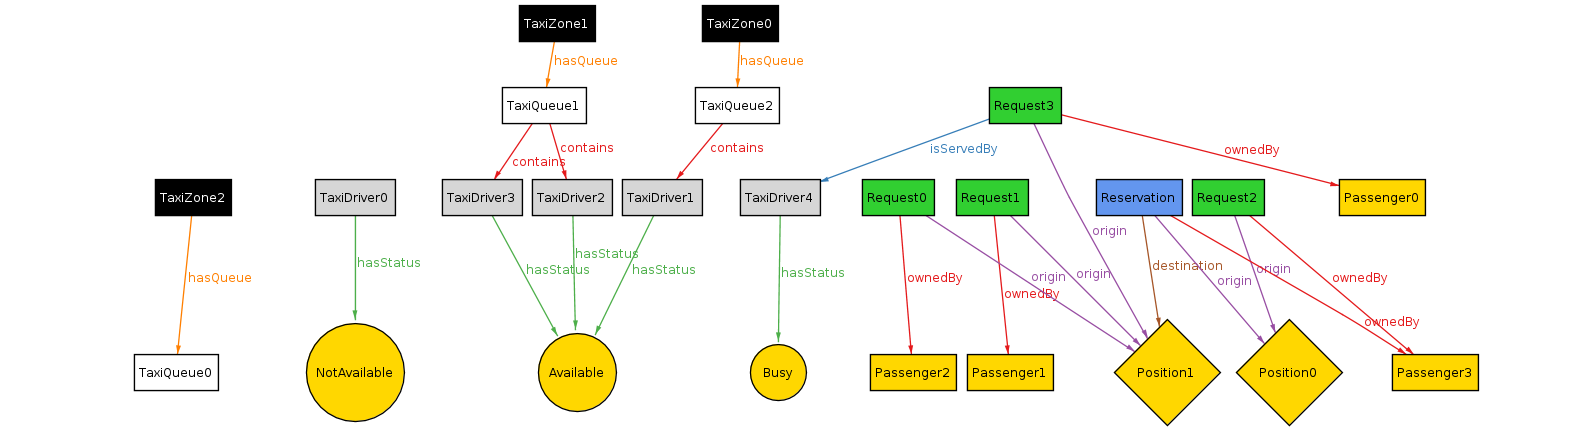
\includegraphics[angle=90, scale=0.5, trim=100 0 180 0]{Appendix/Model}
\end{figure}

\subsection{Notes about the model}
Obviously we did not model all the requirements stated in the previous parts.\\
We mainly used Alloy in the first part of the elicitation of requirements in order to understand the \textbf{main constraints and relations} between the \textit{entities} involved in our problem.\\
For these reasons the model above in of course incomplete and simplified. We are not interested, at this level of abstraction, in modeling every aspect of the system.\\
\\
Our alloy model does not represent the history of the entities involved but a specific point of time. Of course, in the real application, is necessary to provide a support for the storing of information.
